%% content.tex
%%

%% ==============
\chapter{Related Work}
\label{ch:Related Work}
%% ==============

Gesture recognition with wearable devices has been an important research topic over the years. 
There have been a lot of works which used accelerometer-based devices, such as a Wii remote or a data glove. 
Xu, Zhou and Ji experimented with classifying seven hand gestures using the sign sequence of the gesture acceleration as the main feature \todo{[\#]}. 
They tried three different recognition algorithms in order to find the most suitable one. 
The movement data was gathered using MEMS 3-axis accelerometer with a Bluetooth connection to a PC. 
With a dataset of overall 628 samples they achieved an average recognition accuracy of 95.6\% and they concluded, that in this experiment the recognition algorithm based on sign sequence and template matching was the most accurate algorithm. 
Liu also used template matching in order to classify accelerometer data \todo{[\#]}. 
In their experiments, they utilized the three-axis accelerometer from the Wii remote as input device for their classifier. 
They evaluated a large gesture library with over 4000 samples for eight gesture patterns and their results show an overall 98.6\% accuracy and a recognition delay of only 300 ms. 
Kim, Thang and Kim used several accelerometers, with which they created a data glove that was connected via Bluetooth with the PC \todo{[\#]}. 
They performed simple hand gesture recognition by considering a 10-point moving average of the acceleration with which they could achieve a recognition accuracy of 100\% for only three distinct hand gestures. 

Further work has been done focusing on which machine learning algorithm performs best regarding gesture recognition. 
Belgioioso examined acceleration data collected from an iPod Touch and a HTC-Explorer smartphone. 
They experimented based on a dataset of overall 550 samples for four types of gestures and tested classification approaches such as Support Vector Machine (SVM), Relevance Vector Machine (RVM), Sparse Bayesian Learning (SBL) or k-Nearest Neighbor (kNN) \todo{[\#]}. 
For feature extraction, they employed a Principal Component Analysis which is an approach to reduce the dimensionality of a data set consisting of many variables correlated with each other. 
The work concluded that SVM has proved to be the approach with the highest accuracy in recognizing gestures, while SBL based approaches showed comparable classification performances with less computational cost required.
To the best of our knowledge, this work presents the first gesture recognition study using the Thunderboard react.


%% ==============
\chapter{Dashboard}
\label{ch:Dashboard}
%% ==============

The main goal of our seminar work was to implement a gesture recognition program with which we can reliably control applications like dashboards on the computer.
Therefore, we created a test dashboard with which we examined the usability of our program.
It consists of several diagrams which can be modified by steering elements like a dropdown menu and radio buttons.
\todo{The main characteristic of the dashboard is that it can be controlled only with the keyboard buttons “tab”, “up”, “down”, “spacebar”, and “enter”.
This makes the steering with our gesture recognition program easier since we can use the python package “pyautogui” to translate recognized gestures into keyboard commands.}

Of course, this is just a simplified example of a dashboard with only a few features compared to what can be found in actual corporate dashboards which allow more sophisticated commands.
Nevertheless, our dashboard can be easily extended with further features by implementing more steering elements like slide bars or check buttons and by adding more recognizable gestures with which these elements can be controlled.  

\begin{figure}[htp]
\begin{center}
  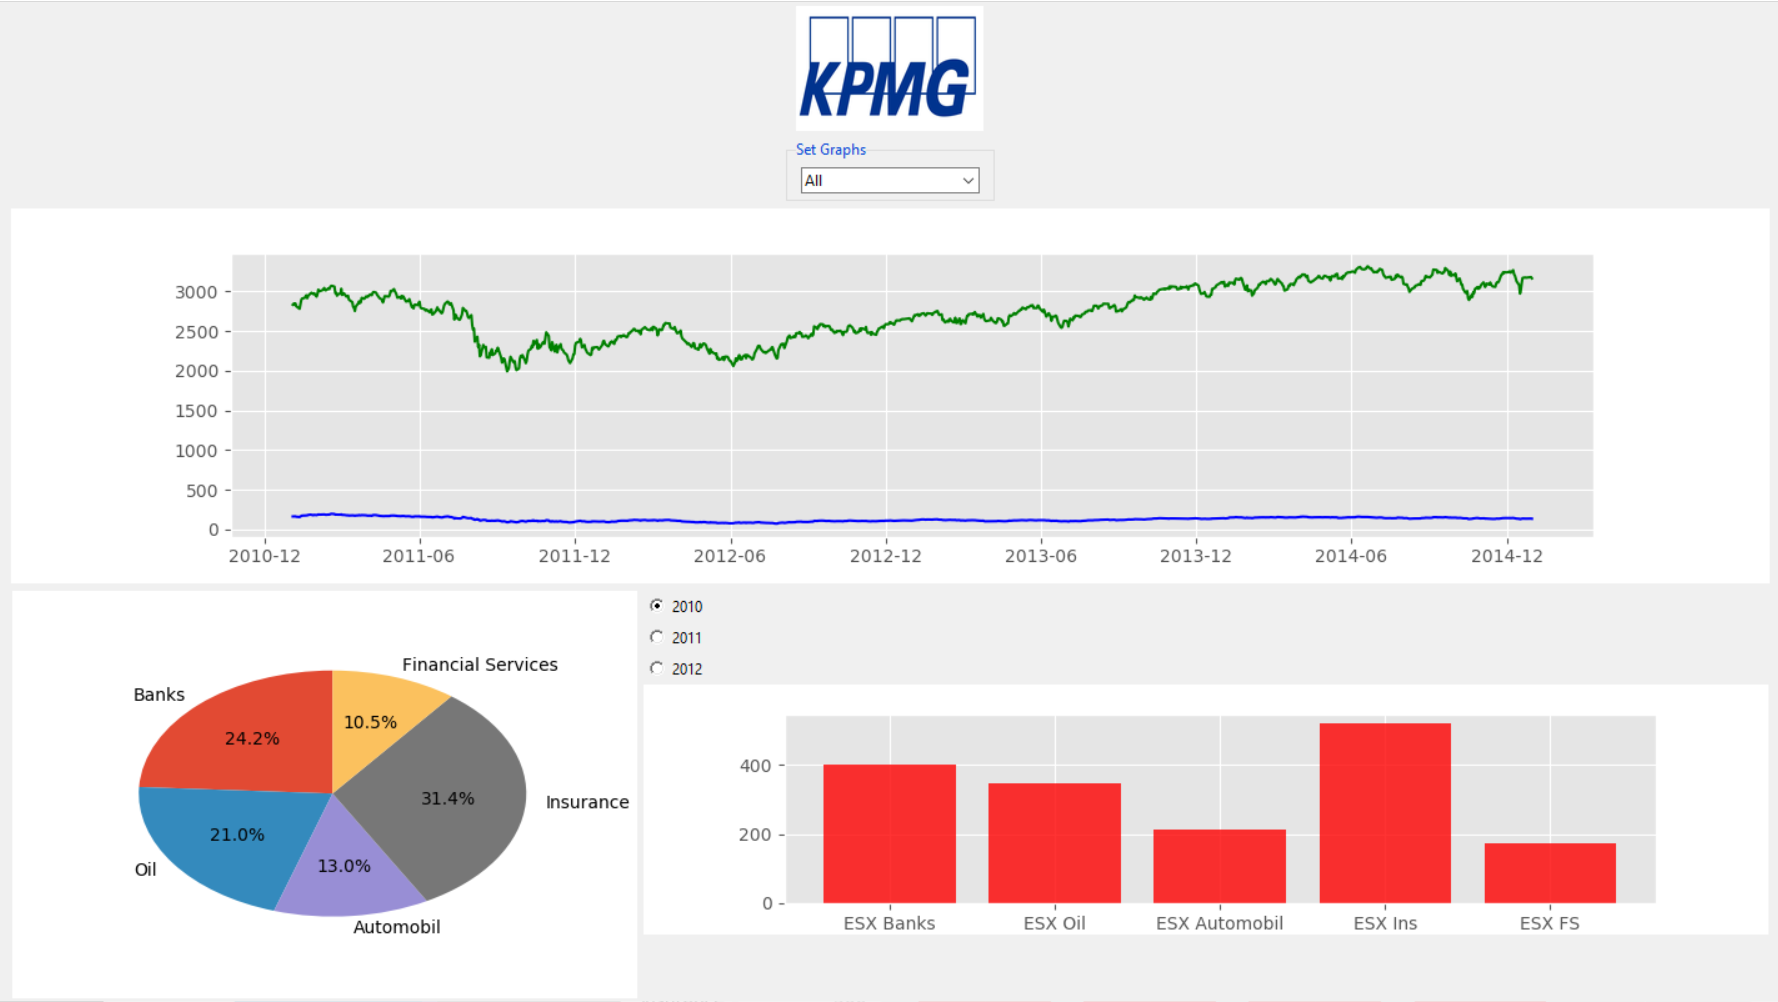
\includegraphics[width = \textwidth]{dashboard.png}
\caption{Our demo application front end}
\end{center}
\end{figure} 


%% ==============
\chapter{System Design}
\label{ch:SystemDesign}
%% ==============

In order to maximize reusability of code we decided to split the app into the six main components shown below. As you can see, our project consists of two individual parts, the recorder app and the recognizer app, sharing two helper modules, labeled Input and Connector. We implemented a core module for each part which is responsible to coordinate data streams and event responses. As such, the core modules instantiate their helper modules and use their interfaces to communicate with them. It is also worth knowing that some modules are divided into multiple files which are documented directly in our code.

%% ===========================
\section{Components}
\label{ch:SystemDesign:sec:Components}
%% ===========================

\begin{figure}[htp]
\begin{center}
  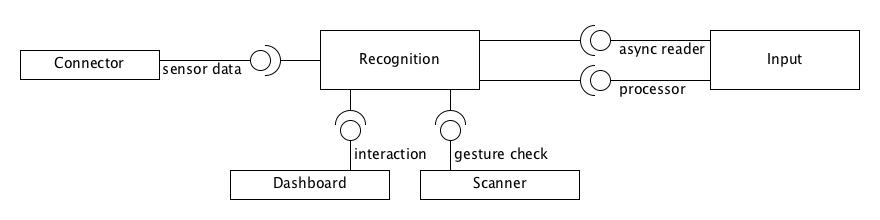
\includegraphics[width = \textwidth]{Component_diagram_recognizer.jpg}
\caption{Recognizer App}
\end{center}
\end{figure} 

\begin{figure}[htp]
\begin{center}
  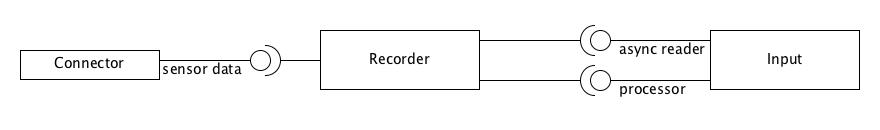
\includegraphics[width = \textwidth]{Component_diagram_recorder.jpg}
\caption{Recoreder App}
\end{center}
\end{figure} 

\newpage

%% ===========================
\subsection{Connector}
\label{ch:SystemDesign:sec:Components:sub:Connector}
%% ===========================

\begin{wrapfigure}{R}{0.5\textwidth}
\centering
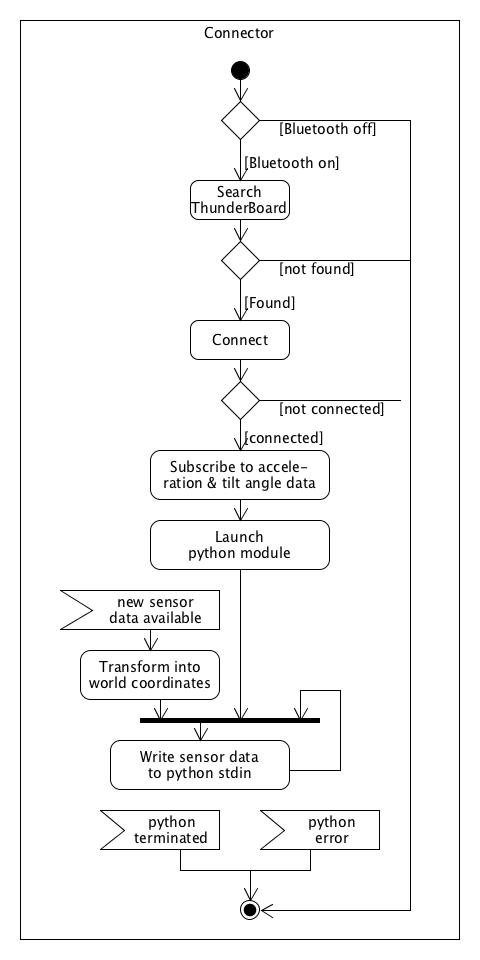
\includegraphics[width=0.5\textwidth]{Connector_flow.jpg}
\caption{Establishing the connection to the Thunderboard React}\label{fig:flow_chart}
\end{wrapfigure}
As we ran into several issues trying to connect the Thunderboard React using Python we implemented the connector in JavaScript and used NodeJS libraries for interfacing the bluetooth device. To launch the recorder or recognizer app you need to launch the connector and pass it the path to the desired core module. After launching the connector it performs the steps shown in the flow chart on the right.

%% ===========================
\subsection{Input}
\label{ch:SystemDesign:sec:Components:sub:Input}
%% ===========================

The input module starts a new thread upon instantiation to avoid blocking the calling thread. In its new thread it keeps reading the sensor data from stdin, parses it into floating point values and inserts them into a ring buffer. Its interfaces can be used to set up the buffer, to reset the buffer, to insert new data into the buffer or to start recording.  In the latter case, the module finds out when the actual gesture started on its own by comparing the acceleration vector length to a threshold value. As soon as the buffer fills up its content is written to a static CSV file autonomously. The input module never takes action on its own but is still smart enough to perform a full control flow to record a gesture or to maintain the ring buffer.

%% ===========================
\subsection{Recorder}
\label{ch:SystemDesign:sec:Components:sub:Recorder}
%% ===========================

The recorder module provides a simple user interface which is used to specify the gesture you want to record as well as to explicitly start recording. That is done through a button which has to be pressed before each single gesture; we implemented it this way in order to avoid accidentally record a gesture which would pollute our training set. It also is responsible for instantiation and hooking up the input module.

%% ===========================
\subsection{Scanner}
\label{ch:SystemDesign:sec:Components:sub:Scanner}
%% ===========================

The scanner module is only used by the recognition module. It is used for monitoring the ring buffer content and for checking whether a gesture was observed. Thus, it instantiates, trains and maintains the machine learning algorithm used to classify live sensor data. Training includes transforming the recorded raw acceleration and tilt angle data into features and feeding them to the machine learning algorithm. All live sensor data will  also have to be transformed into the same features so that they can be classified. We describe what features are and how we transformed the raw data in the next chapter.
To avoid unnecessary complexity, we included the cross validation used to evaluate the performance of different machine learning algorithms directly into the scanner module. Cross validation includes leave one out, 10-fold cross validation and 25-fold cross validation and is performed during instantiation.

%% ===========================
\subsection{Dashboard}
\label{ch:SystemDesign:sec:Components:sub:Dashboard}
%% ===========================

Just like the scanner, the dashboard module is only used by the recognizer app. It provides the user with a user interface showing charts and diagrams based on data by KPMG. That data is read and parsed by the dashboard when it is instantiated. As the user interface provides interactive elements like buttons the dashboard module is also responsible for handling user interaction. In addition, it exposes an interface to the recognition module which is used to broadcast recognized gestures as events to the dashboard. The dashboard can then execute the appropriate action.

%% ===========================
\subsection{Recognition}
\label{ch:SystemDesign:sec:Components:sub:Recognition}
%% ===========================

The recognition module used in the recognizer app is responsible to instantiate and hooking up the input module. It also instantiates the dashboard and implements the logic required to notify it about a recognized gesture.



%% ===========================
\chapter{Data Collection \& Manipulation}
\label{ch:DataCollection}
%% ===========================

Working  with  machine  learning  algorithms  requires  certain  actions  in  order  to choose, prepare and classify data streams.
Choosing the right data is the key decision in order to be able to train the  algorithm properly.
In addition to this  step, preparing data and transforming it into “features” is equally important. 

%% ===========================
\section{Data Collection}
\label{ch:DataCollection:sec:DataCollection}
%% ===========================

To  define  which  data  will  be  collected  we  had  to  think  about  which  kind  of gestures  we  will  want  to  recognize.
Attaching  the  sensors  to  the  back  of  our  hand enables us to observe acceleration data  for x,  y, and z axis  as well  as tilt  angles  alpha, beta and gamma.
We thought about attaching a magnet to our thumb so that we can use the hall-sensor as well,  but we decided to leave this  for  further research.
The collected acceleration and tilt angle data can later be used to distinguish gestures from each other.
To avoid recording and scanning data observed during normal gesticulation we require the acceleration vector length of each gesture to exceed a certain threshold.
In our code we set this treshold to 1.2 G.

%% ===========================
\section{Feature Design}
\label{ch:DataCollection:sec:FeatureDesign}
%% ===========================

Before we can train our algorithm, we  have to transform the recorded data into a set  of  features.
Choosing  and  designing  those  features  affects  the  performance  of  the gesture recognition algorithm heavily.

%% ===========================
\subsection{Preprocessing}
\label{ch:DataCollection:sec:FeatureDesign:sub:Preprocessing}
%% ===========================

Standardization,     scaling,     normalization     and     binarization     are     common preprocessing techniques.
Though, as the acceleration vector and tilt angel sizes are key characteristics  to  distinguish  gestures  scaling,  normalization  and  binarization  are  not applicable for our use case. 

%% ===========================
\subsection{Features}
\label{ch:DataCollection:sec:FeatureDesign:sub:Features}
%% ===========================

\todo{Add images of feature selection}
We  first  thought  about  using  the  variance  as  a  feature,  but  early  tests  already revealed  that  the  acceleration  data  often  has  a  variance  near  zero  and  thus  gives  us almost no information about the executed gesture.

Instead,  maximum  and  minimum  acceleration  per  axis  differ  widely  across gestures  and  are  worth  adding  to  our  feature  set.
To give our classifier a idea of which minimum/maximum was the first, we put them in the right order, so if we have a maximum first, this will be the first feature and the miniumum will become the second feature.
For  instance,  swiping  left  first  shows  a negative  minimum  acceleration, e.g. -1.7G, and then a positive  maximum acceleration, e.g. 1.2G, on the x axis.
We now pick those values out of our buffer and figure out which one was earlier, so we can put them in our feature vector in the right order.
In  this example, we end up with the tuple (-1.7, 1.2).

To include the tilt angles into our feature set, we had to come up with a different approach.
Not only was their variance near zero, but also their minimum and maximum values  are  often  equally  great  across  different  gestures. 
Summing  up  all  angles  led  to non-satisfying  results,  so  we  collect  now  two  features  per  angle:
One  sums  up  the absolute  values  of  negative  angle  differences  and  the  other  one  sums  up  the  absolute values  of  the  positive  angle  differences.
Comparing  both  approaches  the  latter  one increased our average precision  score by ~6\%.
\todo{Include stats “First Approach” vs “Final Solution” here}

%% ===========================
\section{Data Classification}
\label{ch:DataCollection:sec:DataClassification}
%% ===========================

Depending on the underlying training set, each classifier performs a bit different. We tested the K-Neighbors classifier with five and eleven nearest neighbors, Random Forest classifier with 10 and 100 estimators,  Decision Tree classifier, Support Vector Machine and Gaussian Bayes, which is a neural network. We then created a Voting classifier based on the two best classifiers to push the limits even further. Each classifier was evaluated with leave one out and 25-fold cross validation techniques, the results are summarized in the diagrams below:
%% \todo{Discuss which classifier we took, based on stats


\begin{figure}[!htb]
\minipage{0.32\textwidth}
  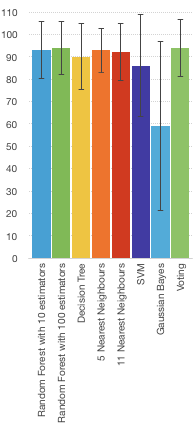
\includegraphics[width=\linewidth]{25fold_cv_precision.png}
  \caption{25-fold cross validation precision}\label{fig:precision}
\endminipage\hfill
\minipage{0.32\textwidth}
  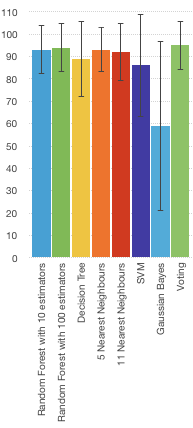
\includegraphics[width=\linewidth]{25fold_cv_accuracy.png}
  \caption{25-fold cross validation accuracy}\label{fig:accuracy}
\endminipage\hfill
\minipage{0.32\textwidth}%
  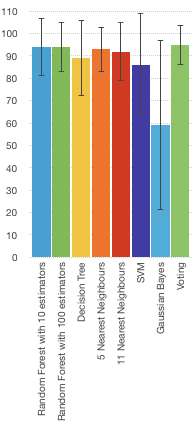
\includegraphics[width=\linewidth]{25fold_cv_recall.png}
  \caption{25-fold cross validation recall}\label{fig:recall}
\endminipage
\end{figure}

As you can see, the Gaussian Bayes and Support Vector Machine perform poorly compared to the other classifiers. Both their expectancy value and their standard deviation are unfavourable for practial use. In contrast, the Decision Tree classifier reaches almost 90\% precision, accuracy and recall expectancy value. The prediction is based on a tree; inputs always iterate through each node until they reach a leave. Each node checks and classifies the input values and has one incoming and two outgoing edges. The leaves finally state which gesture the input data corresponds to. Using a tree is apparently a propmising solution, but as we end up in a leave the prediction has always a probability of 100\% which limits this classifiers abilities to some extent. Combining multiple trees by using a so called Random Forest led to much better results. As shown in the diagram, the expectancy value of our classifier with 100 estimators reaches 94\% precision, accuracy and recall. 

\begin{wrapfigure}{R}{0.4\textwidth}
\centering
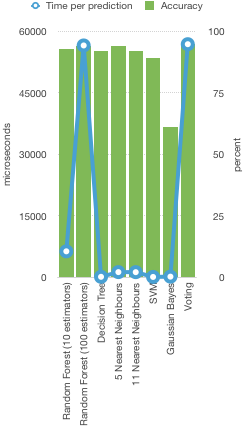
\includegraphics[width=0.4\textwidth]{loo_cv.png}
\caption{Leave one out cross validation accuracy}\label{fig:loo}
\end{wrapfigure}

The K-Neighbors classifier follows a differnet approach. Simply put, training data is mapped into a coordinate system. Input data is then mapped the same way and classified by checking the K nearest training data points in that coordinate system relative to the input data. Whatever gesture the majority of these K neighbors is assignet to is the predicted gesture of our input. In our case K was five or eleven. Considering just 5 neighbors showed off to be the better solution and compares very vell to our Desicion Tree classifier with 100 estimators: The K-neigbors classifier performs about 1\% worse, but has a much smaller standard deviation equal to 10\% in precision, accuracy and recall instead of 11\% - 13\%.

Having examined those common classifiers we combined the two best of them, Random Forest with 100 estimators and 5-Neighbors, into a Voting classifier. Tests revealed that giving the Random Forest predictions twice the weight of the 5-Neigbors predictions increases the expectancy value of our Voting classifier to 95\% accuracy and recall while slightly decreasing the standard deviation. Due to these observations we decided to use the Voting classifier to control the dashboard.

In order to provide a convenient user experience gestures need to be predicted fast enough during app usage. We meassured the average prediction time for each classifier during our leave one out cross validation. The results are presented in figure \ref{fig:loo} and justify our decision to use the Voting classifier for production. Although it has the highest prediction time we think that fiftysix milliseconds are still appropriate for real world applications. What is also worth noting is that the 5-Neighbors classifier needs approximately one millisecond and still performs almost as well as the Random Forest classifier with 100 estimators. So the relatively large prediction time of the Voting classifier is mainly caused by the Random Forest classifier we applied to the classifier set.

